\documentclass[12pt,a4paper]{article}
\usepackage[utf8]{inputenc}
\usepackage{graphicx}
\usepackage{amsmath}
\usepackage{amsthm}
\usepackage{amssymb}
\usepackage{hyperref}

\begin{document}

\begin{titlepage}
	\centering
	
\includegraphics[width=0.15\textwidth]{IIIT-B_logo.jpg}\par\vspace{1cm}
	{\scshape\LARGE International Institute of Information Technology Bangalore \par}
	\vspace{1cm}
	{\scshape\Large Software Design Document\par}
	{\Large DS 703 Geographic Information Systems\par}
	\vspace{1.5cm}
	{\huge\bfseries Multimodal Route Planning\par}
	\vspace{2cm}	   
	{\Large\itshape Anoop Toffy - MT2016016\par}
	{\Large\itshape Harshit Joshi - MT2016059\par}
	{\Large\itshape Mehul Singh - MT2016083\par}		 	 
	{\Large\itshape Mohammad Awais - MT2016086\par}
	\vfill
	Guide : \par
	Dr. S. Rajagopalan

	\vfill

% Bottom of the page
	{\large \today\par}
\end{titlepage}


\tableofcontents
\listoffigures
\listoftables
\newpage

\section{Problem Description}
For a traveller it is often reliable when it comes to use different modes of transport for a single travel whenever it is available. But there lacks efficient systems to find out, even though there are systems that aid traveller to choose different modes of transport, such as Google Transit. \\
Multimodal Route Planning(MRP) is system that provides the traveller with optimal, feasible and personalized route plan between a given source and destination. The system is designed to provide various public travel approaches (like bus riding, metro travel) and provides traveller the flexibility to choose from different modes of transport.


\section{Data Collection and Preprocessing}

The bus and metro schedules are collected from the Bengaluru Metropolitan Transport Corporation (from GPS records) and Bengaluru Metro departments. It is then represented as graphs (transportation networks) from the longitude and latitude data. The graphical representation of unimodal networks are done using software's likes qgis. 

\section{Building the multimodal network model}



\subsection{unimodal network construction}

\subsubsection{Bus network model}
The bus network model is build from the co ordinates of the bus stops obtained from the data collected from bmtc. It is then fed into the software like Qgis to build a unimodal graph network.

\subsubsection{Metro network model}
The metro network modal is build from the GPS records of the metro network. A unimodal graph network is constructed from it using software like Qgis.

\subsection{Merging and linking to form multimodal network model}

\subsubsection{Merging}

The merging operation is performed using nearest neighbour algorithm. It uses linear search to find out the nearest location in the given two unimodal network considered for merging.

\subsubsection{Linking}

The unimodel network that are being merged are linked by two types of link, walk\_link or bicycle\_link for the completion of multimodel network model. The walk\_link or bicycle\_links are added based on the shortest harvesine distance (for a predefined threashold, $T_{d}$) for a transit between the two modes of transport.

\begin{figure}[!hp]
    \centering
    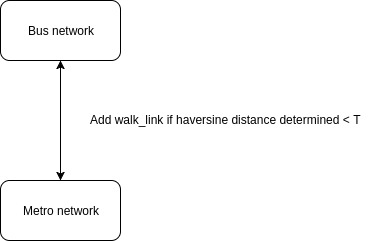
\includegraphics[width=0.8\textwidth]{flowcharts/linkaddition.jpg}
    \caption{Add link if its less than a Threshold, T}
    \label{fig:Enduser flow}
\end{figure}

\section{Algorithm for multimodal route planning}

In the simplest form the algorithms for journey planning is a shortest path problem from the given start location to the destination. MRP helps traveller combine various modes of transport like bus riding and metro travel for a single trip by using heuristics approach. 

The algorithm proposed here uses $A^{*}$ graph search with acceptable heuristics(Expected time of Travel, ETA estimated from historical data) to provide a deterministic solution to mutlimodal routing problem from the multimodal transportation network data gathered from merging unimodal graph networks. The general solution is NP Hard since there is always a level of non determinism for example. boarding of the bus (can succeed or fail).

In MRP there are multiple quality criteria such as travel time, number of interchanges, cost etc.

\subsection{$A^{*}$ Graph Search with Admissible Heuristics}

The step by step approach for solving the multimodal routing problem is as follows:

\begin{itemize}
\item Build the unimodal network for each modality of transport. (here, for bus network, metro network).
\item Merge unimodal network using nearest neighbour and link the unimodal network using alternative means of travel like (walking, cycling etc)
\item Apply $A^{*}$ graph search to find the shortest path between given destination from the traveller location.
\end{itemize}

\subsubsection{Admissible Heuristics}
We uses Expected Time of Travel (ETA) from historical data as a admissible heuristic metric.

\subsection{Input description}
The spatial data can be plotted on OpenStreetMap or Google Maps using WGS 84 datum via softwares like QGIS and corresponding network is generated from it. This network is used to find the shortest feasible route to travel from a given location.

\subsection{Algorithms}
The algorithm use probabilistic heuristics to find out optimal path between source and destination by incorporating various modes of travel selected by the traveler.

\subsection{Output}
An optimal route is returned by the system as the output.

\newpage

\section{Flow Diagrams}

\subsection{End user flow}
\begin{figure}[!hp]
    \centering
    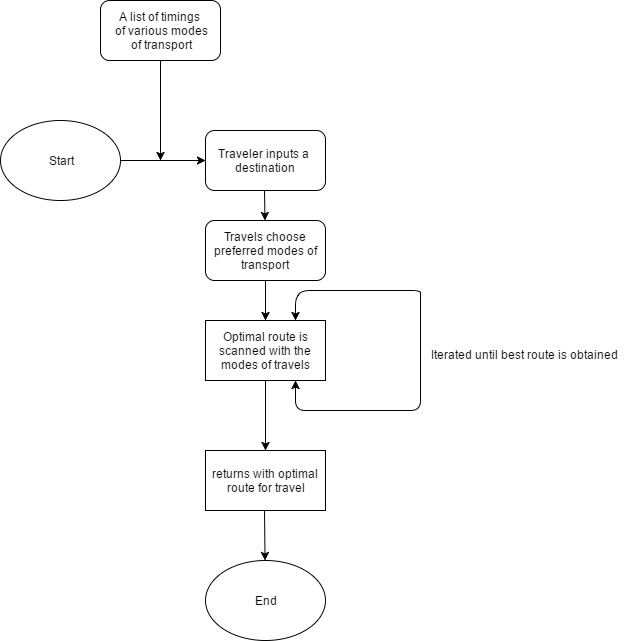
\includegraphics[width=1.25\textwidth]{flowcharts/basicflow.jpg}
    \caption{End user}
    \label{fig:Enduser flow}
\end{figure}

\newpage

\subsection{Back end flow}

\begin{figure}[!hp]
    \centering
    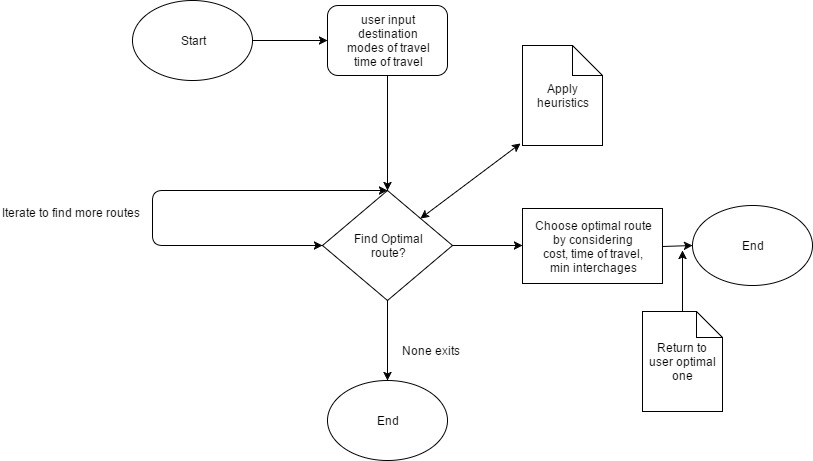
\includegraphics[width=1.25\textwidth]{flowcharts/backend.jpg}
    \caption{backend}
    \label{fig:backend flow}
\end{figure}

\end{document}